\documentclass{emulateapj}
\usepackage[colorlinks,urlcolor=blue,citecolor=blue,linkcolor=blue]{hyperref} 
\usepackage{graphicx,natbib}
\citestyle{aa}
\usepackage[space]{grffile}
\usepackage{latexsym}
\usepackage{amsfonts,amsmath,amssymb}
\usepackage{url}
\usepackage[utf8]{inputenc}
\usepackage{fancyref}
\usepackage{hyperref}
\usepackage{multirow}
\hypersetup{colorlinks=false,pdfborder={0 0 0},}

\newcommand{\rf}{\emph{realfast}}
\newcommand{\frb}{FRB 121102}

\begin{document}

\title{\frb: Properties of VLA Bursts and Implications for Overall FRB Population}
\shorttitle{\frb\ Burst Properties}
\shortauthors{Law et al.}

\author{Casey J. Law\altaffilmark{1}}
\author{Dewey}
\author{Cheetham}\author{Howe}
\altaffiltext{1}{Dept of Astronomy and Radio Astronomy Lab, Univ. of California, Berkeley, CA}

\begin{abstract}
The millisecond radio transients known as Fast Radio Bursts have recently emerged as a mysterious, new class of astrophysical transient. The discovery of repeating bursts from \frb\ has shown that at least some FRBs are not cataclysmic and opened potential for studying a FRB properties via a homogenous sample of bursts. With the recent localization of \frb with the Very Large Array has helped measure its distance and intrinsic properties of the bursting source and its multiwavelength associations. This localization was made with 9 bursts seen by the VLA in coordination the Arecibo, Effelsberg, and AMI-LA observatories. We present a detailed analysis of these bursts, including the first simultaneous detection of an FRB with multiple telescopes. We show that the burst spectra typically have a broad Gaussian shape on the scale of $\sim500$~MHz with fine spectral structure consistent with either scintillation or nanosecond temporal structure. We present the first burst flux distribution and temporal statistics for \frb and argue that it is consistent with the broader FRB population...
\end{abstract}

\section{Introduction}
Fast Radio Bursts (FRBs) are a new class of millisecond-duration radio transient with a dispersion measure (DM) that implies that they originate outside of our Galaxy. At extragalactic (and potentially cosmological) distances, they are not only unusually luminous, but they provide a new tracer of other galaxies and the intergalactic medium (IGM). In this way, FRBs have opened a whole new playground in astrophysics \citep[e.g.,][]{2014A&A...562A.137F, 2014ApJ...780L..33M, 2016MNRAS.457..232C}. However, that potential has been hamstrung by the lack of a definitive association of an FRB to an extragalactic host.

This paper is part of a series that presents the first localization and host identification of an FRB (CITE, CITE, ...). \frb, also known as the ``repeating FRB'', was first detected in November 2012 by the Arecibo Observatory \citep{2014ApJ...790..101S}. In mid 2015, new Arecibo observations revealed a series of bursts at the same DM and sky position demonstrating that FRBs are capable of repetition \citep{2016Natur.531..202S}. Beginning in August of 2015, we made the first of nine detections of \frb\ with the Very Large Array (CITE) and localized it with a precision of 0.1\arcsec. Deep radio and optical observing shows that \frb\ is unambiguously associated with a persistent radio and optical source at a redshift of 0.193 (CITE).

\frb\ has now been localized three orders of magnitude better than any other FRB and placed at a cosmological distance. Its lookback and luminosity distances are 746 and 972 Mpc \citep{planck15}, which are orders of magnitude larger than any other millisecond transient. This shows that FRBs:
\begin{itemize}
 \item are extremely luminous, 
 \item have a significant DM contribution from the IGM, and
 \item can be used to probe the IGM and their host galaxy.
\end{itemize}
The promise implied by the first reported FRB \citep{2007Sci...318..777L} is now being realized.

The cosmological distance for \frb\ could have wide-ranging implications for the FRB population as a whole. However, it has not been demonstrated that \frb\ is representative of the overall FRB population. In fact, the repetition of its bursts is unique among all FRBs \citep{2015MNRAS.454..457P}, so it is natural to ask whether \frb\ is representative. An important first step is to demonstrate that the properties of \frb\ are consistent with the significant body of facts for the overall population \citep{2015MNRAS.451.3278M, 2016MPLA...3130013K}. The repeating nature of \frb\ provides us with several statistical tests we can use to test this connection.

We can also assume that \frb\ is representative and use it to constrain the physical processes at play in the overall FRB population. Although we now know that FRBs are luminous, it is not yet clear what process generates the radio bursts themselves \citep{2014PhRvD..89j3009K, 2014ApJ...785L..26L, 2016MNRAS.457..232C}. The simultaneous \frb\ observing campaign with the VLA, Arecibo, Effelsberg, GBT, and AMI-LA gives a more complete picture of the spectral structure of FRB radio emission. FRB repetition also has strong implications for the number of FRB-generating systems in the universe \citep{2016MNRAS.458L..89C}.

Given that FRBs are now known to be useful probes of the IGM, there is strong justification for continuing searches for new detections and localizations. The relatively faint counterpart to \frb\ argues that direct localization of the radio burst will continue to be the best way to find optical hosts to measure distances. Our multi-telescope constraints on burst spectra, measurement of host properties, burst rate estimates, and other properties will inform new strategies for finding FRBs...

\section{Observations}

\begin{figure*}[t]
\begin{center}
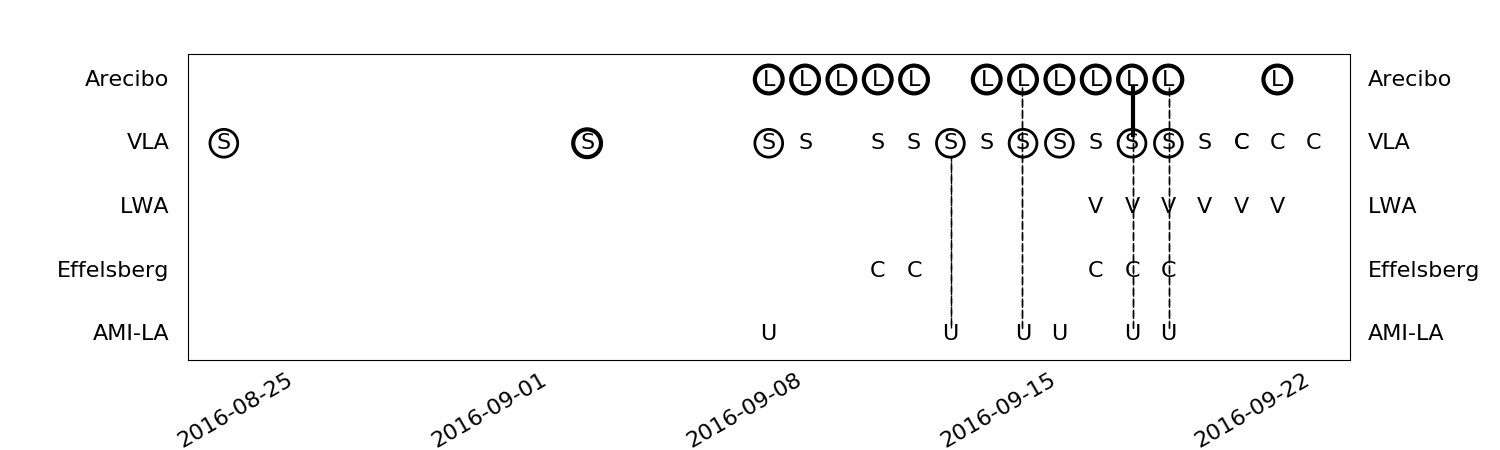
\includegraphics[width=2\columnwidth]{timeline}
\caption{Summary of observing coverage and detections of \frb\ during the multi-telescope observing campaign. Symbols show days with observations and symbols with circles show detections of \frb. Multiple circles indicate multiple burst detections, except for Arecibo, which typically has multiple detections per observing session (a detailed analysis is left for a future paper). The black dashed lines show the VLA burst detections with simultaneous coverage at other telescopes. The solid black line shows the simultaneous burst detection at VLA and Arecibo.
\label{fig:multi}}
\end{center}
\end{figure*}

The data presented here were obtained from multiple programs and telescopes, but the central goal was to interferometrically localize \frb\ with the VLA. The observing strategy was to ensure simultaneous observing between the VLA and Arecibo observatories and add other observatories added on a best-effort basis. The hope was that Arecibo could be used to define times of bursts for which we could selectively search with the VLA. This would reduce the trials factor that limited sensitivity and potentially provide detections at multiple independent bands. Below, we summarize these observations, with a focus on those conducted simultaneous with VLA burst detections from \frb.

\subsection{VLA}
The \frb\ observing campaign started in late 2015 with a 10~hr campaign observed at 1.4~GHz in the compact D configuration. In April through May 2016, we conducted a 40~hr campaign at 3.0~GHz in the C and CnB configurations in coordination with Arecibo. We concluded with a new, 40~hr, coordinated campaign from August through September 2016 in the B configuration and during the move to the most extended A configuration. In this last campaign, the first 34 hours of VLA observations were made at 3.0~GHz, while the last 6 hours were observed at 6~GHz.

All VLA fast-sampled data were observed with 5~ms sampling, 256 channels, and dual-circular polarization \citep[as in]{2015ApJ...807...16L}. To maximize sensitivity, the channel frequency width was set to maintain sensitivity to the known DM of \frb, while maximizing the total bandwidth. The total bandwidth at L (1.4~GHz), S (3.0~GHz), and C (6.0~GHz) bands was 256~MHz, 1.0~GHz, and 2.0~GHz, respectively.

Observations in August and Septmeber were searched by a prototype version of \rf\footnote{See \url{http://realfast.io}.}. \rf\ is a real-time, fast imaging transient search system. The current, prototype runs on existing, CPU-based hardware of the VLA correlator backend, while the future \rf\ will run on a dedicated GPU cluster. The transient search pipeline software is called ``rtpipe''\footnote{See \url{https://github.com/caseyjlaw/rtpipe}} and is mostly written in Python. The transient search pipeline is described in \citet{2015ApJ...807...16L} and performs data calibration, flagging, dedispersion, and imaging. Images were formed for each integration at DMs of 0, 546, 556.9, 560, and 565 pc cm$^{-3}$. Gain calibration is read from the "telcal" system, which uses phase-only calibration on the previous gain calibrator.

Burst detections and localizations were made within hours of data being recorded. The transient search starts when data are recorded, but this prototype of \rf\ is a factor of several times slower than real-time, so we refer to the detection as "quasi real-time". Each image with a pixel higher than 6.4$\sigma$ has some rudimentary data saved to capture both real and thermal-noise candidates as a check of data quality. For each image with a pixel higher than 7.4$\sigma$, \rf\ generates a candidate visualization with an image and spectrum. More detailed analysis, including improved calibration and localization, is conducted offline. 

Computational notebooks to reproduce the transient detection and localization can be found at \url{https://github.com/caseyjlaw/FRB121102}. Time cut-out visibility data are available at \url{https://doi.org/10.7910/DVN/TLDKXG}. Original visibility data are available under VLA program codes 16A-459 and 16A-496 and can be downloaded at \url{http://archive.nrao.edu}.

\subsection{Arecibo}

% copied from the first paper
During the joint Arecibo-VLA campaign, Arecibo observed with the L-wide receiver, which has an observational frequency range of 1.15 to 1.73~GHz and a full width at half maximum beam size of 3.3 arcmin. The PUPPI pulsar backend was used to record total intensity spectra with time and frequency resolutions of 10.24~$\mu$s and 1.5625~MHz, respectively, and full Stokes polarization information. Each frequency channel was coherently dedispersed to 557 pc cm$^{-3}$, thereby eliminating intra-channel dispersion smearing. PUPPI covers a total of 800~MHz of bandwidth centred at 1380.78125~MHz, but only $\sim$ 620~MHz of this band is usable due to radio frequency interference and receiver sensitivity roll-off at the band edges.

4 observations during VLA bursts... One simultaneous detection. Lots more activity at Arecibo overall.

\subsection{Effelsberg}

% copied from Laura's paper
Observations were conducted at an observing frequency of 4.6 to 5.1~GHz. The S60mm receiver has a system equivalent flux density of 18 Jy and a full-width half-max (FWHM) beam size of 2.4\arcmin at 4.85~GHz. Pulsar search mode data were recorded with the PFFTS backend. Total intensity spectra were recorded with a time resolution of 65.5~$\mu$s and a bandwidth of 500~MHz divided into 128 frequency channels. Due to a configuation error, a filter was added that limited the bandwidth to 100-MHz filter centered on 4.85 GHz for Sept 16--18. Note, the inter-channel DM smearing time for 560~pc cm$^{-3}$\ is $\sim$0.2 msec at 4.6 GHz.

100~MHz BW filter in place for two sessions coincident with VLA...

2 observations during VLA bursts...

\subsection{AMI}

4 observations during VLA bursts... Upper limit on burst flux density limits any significant "afterglow". Deep image sensitivity is limited by confusion and is approximately equal to the flux density observed by VLA (CITE).

\section{Results}

\subsection{VLA Bursts}

\subsubsection{Dynamic Spectra}
Figure \ref{fig:sgram} shows the spectrograms of all nine bursts detected by \rf.

\begin{figure*}[htb]
\begin{center}
 \begin{minipage}{2\columnwidth}
  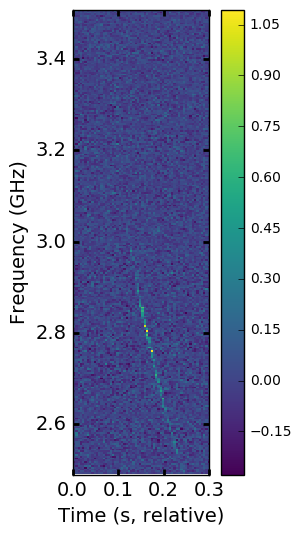
\includegraphics[width=0.25\columnwidth]{sgram_57623.png}
  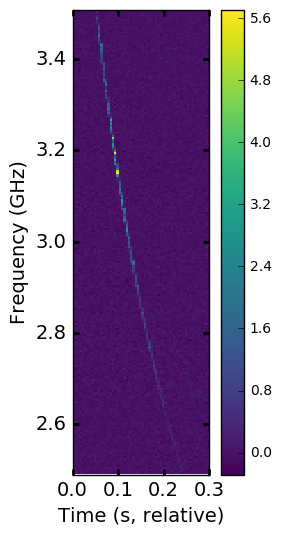
\includegraphics[width=0.25\columnwidth]{sgram_57633_scan7.png}
  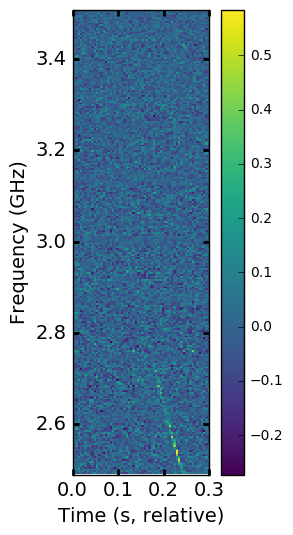
\includegraphics[width=0.25\columnwidth]{sgram_57633_scan13.png}
 \end{minipage}

 \begin{minipage}{2\columnwidth}
  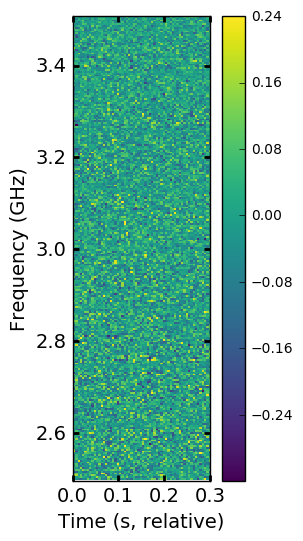
\includegraphics[width=0.25\columnwidth]{sgram_57638.png}
  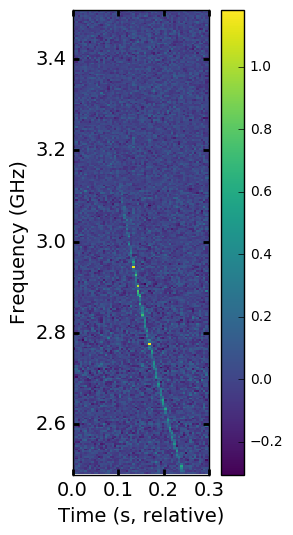
\includegraphics[width=0.25\columnwidth]{sgram_57643.png}
  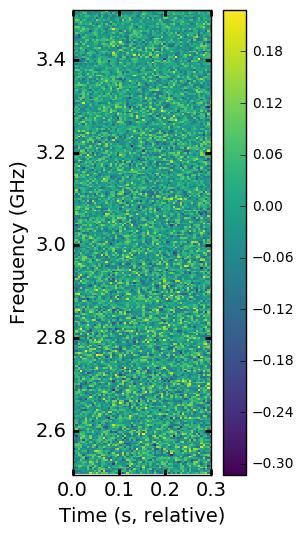
\includegraphics[width=0.25\columnwidth]{sgram_57645.png}
 \end{minipage}

 \begin{minipage}{2\columnwidth}
  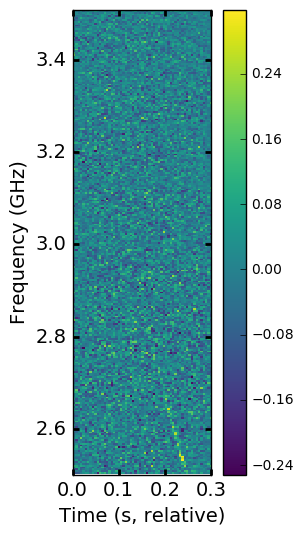
\includegraphics[width=0.25\columnwidth]{sgram_57646.png}
  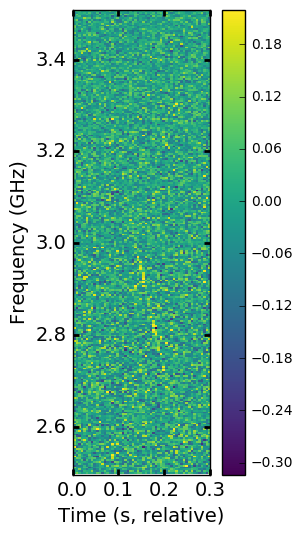
\includegraphics[width=0.25\columnwidth]{sgram_57648.png}
  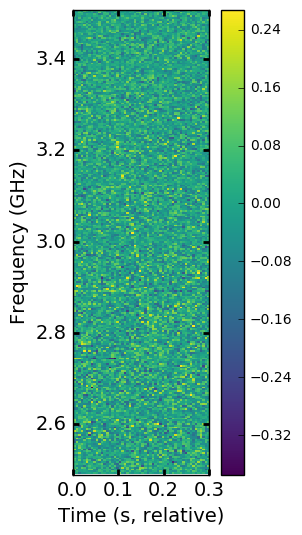
\includegraphics[width=0.25\columnwidth]{sgram_57649.png}
 \end{minipage}
 \caption{Spectrograms (time vs frequency intensity maps) for all nine VLA bursts. Note that bursts are detected in 5~ms images generated from dedispersed visibilities.
 \label{fig:sgram}}
\end{center}
\end{figure*}

We used a fine dispersion grid to find the best-fit DM for each burst. Table \ref{tab:spec} shows the best-fit DM values... Dispersion measure changes between bursts significant?

\begin{table}
\caption{Spectral Modeling of Bursts}
\centering
\begin{tabular}{llll}
\hline
Burst & Peak & Center & Width \\
(MJD) & (Jy *not normed yet*) & (ch) & (ch) \\ \hline
57623 & 33 & 69 & 32 \\
57633, scan 7 & 260 & 163 & 55 \\
57633, scan 13 & & & \\
57638 & & & \\
57643 & 55 & 69 & 56 \\
57645 & & & \\
57646 & & & \\
57648 & & & \\
57649 & & & \\ \hline
\end{tabular}
\label{tab:spec}
\end{table} 

\subsubsection{Spectral modeling}
After detection, we refined the analysis of each burst offline. Burst spectra are shown in Figure \ref{fig:spec}...

\begin{figure*}[h!]
\begin{center}
 \begin{minipage}{2\columnwidth}
  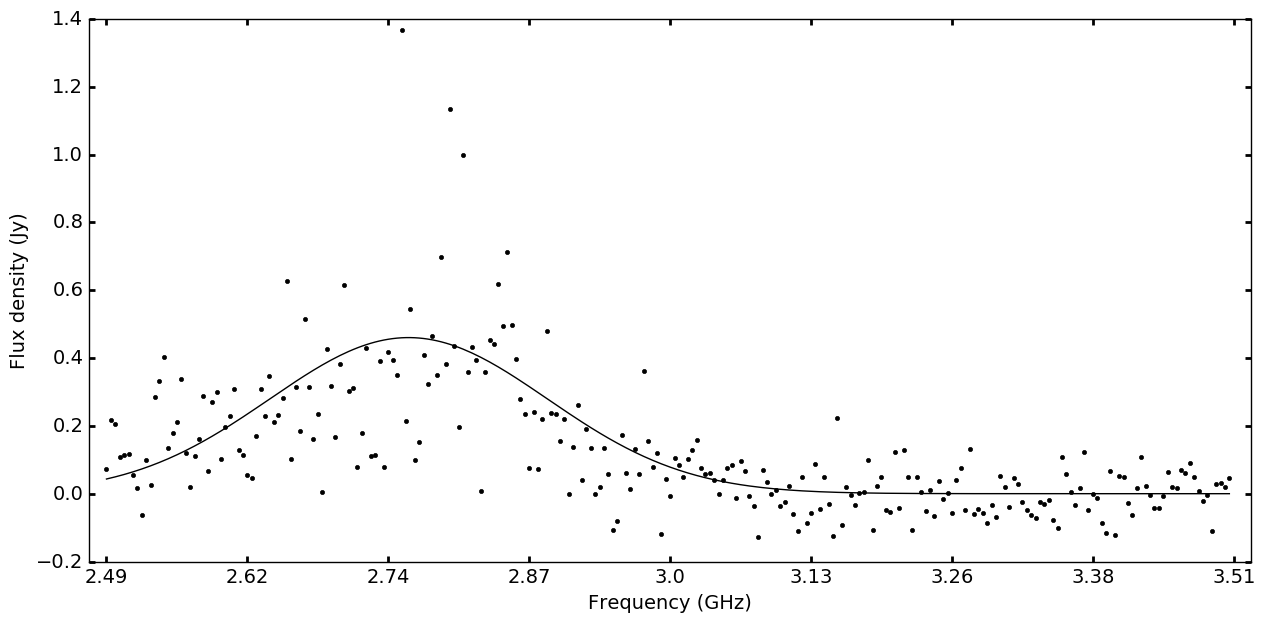
\includegraphics[width=0.3\columnwidth]{spec_57623.png}
  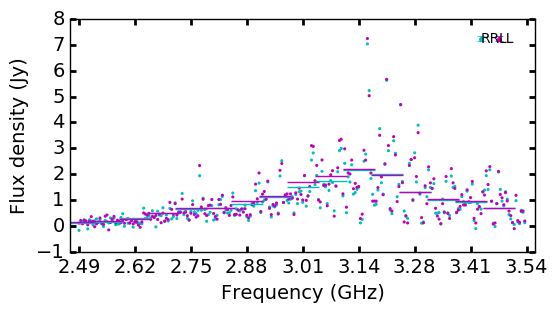
\includegraphics[width=0.3\columnwidth]{spec_57633_scan7.png}
  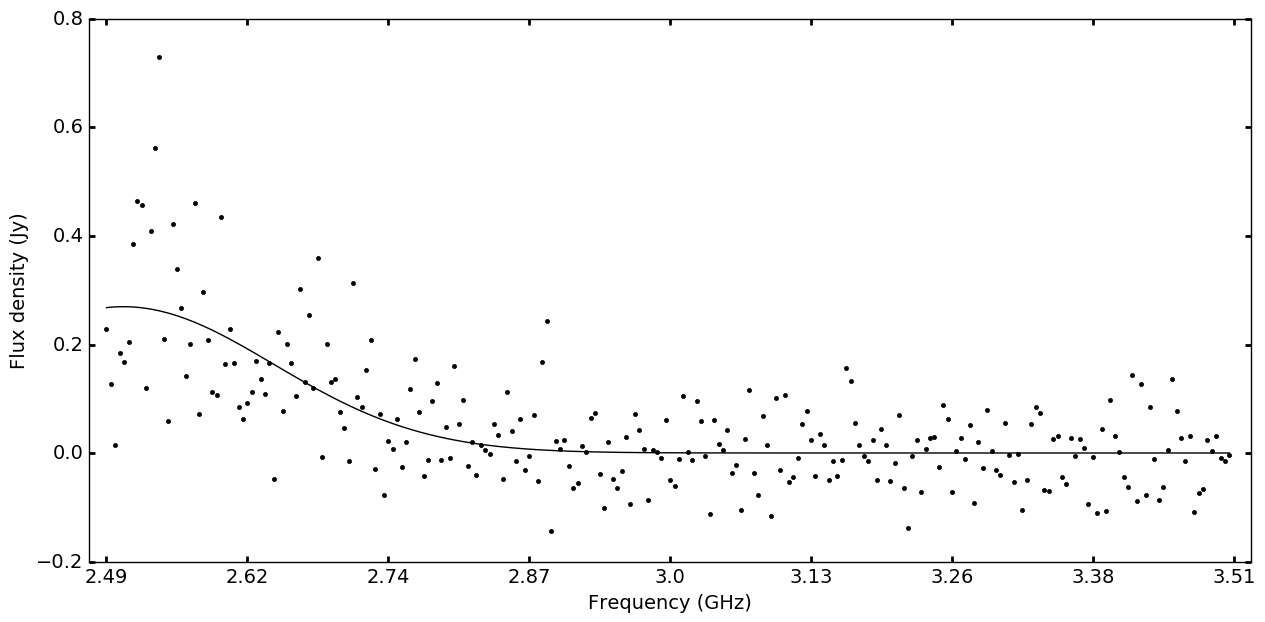
\includegraphics[width=0.3\columnwidth]{spec_57633_scan13.png}
 \end{minipage}

 \begin{minipage}{2\columnwidth}
  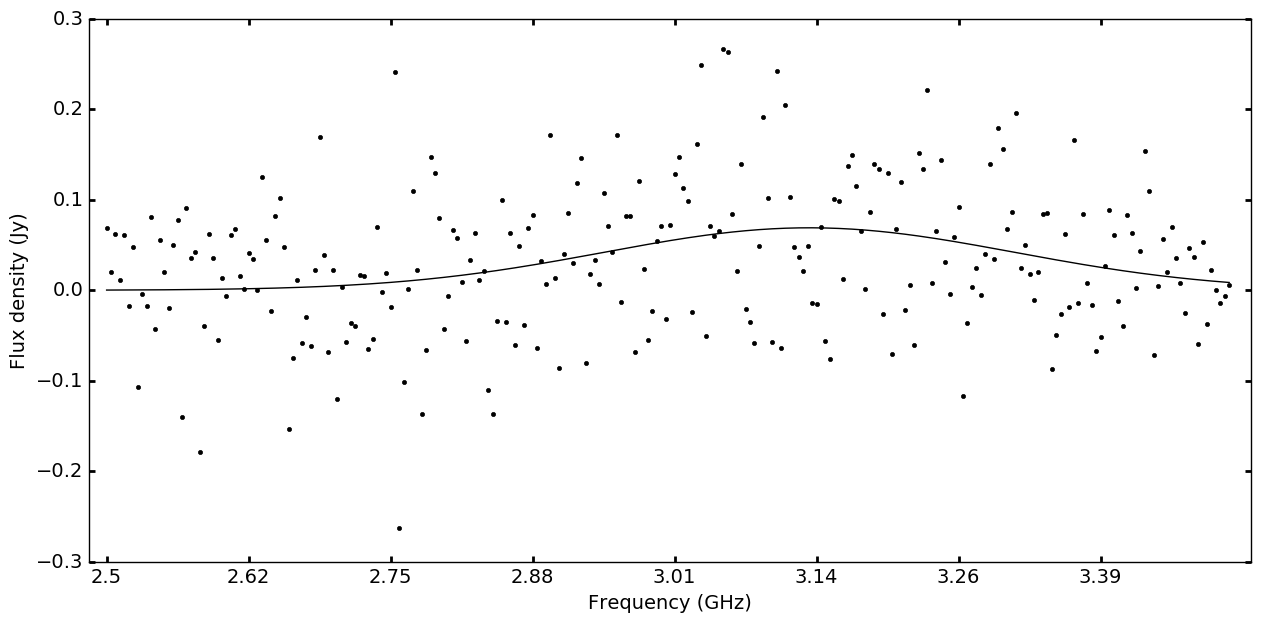
\includegraphics[width=0.3\columnwidth]{spec_57638.png}
  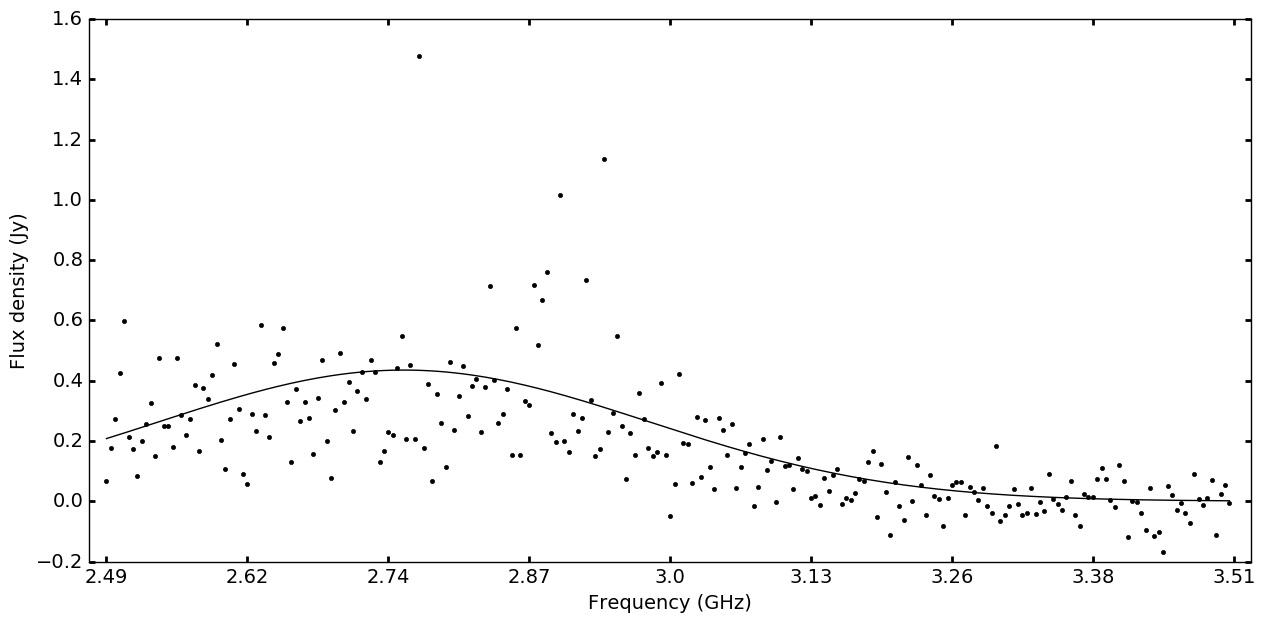
\includegraphics[width=0.3\columnwidth]{spec_57643.png}
  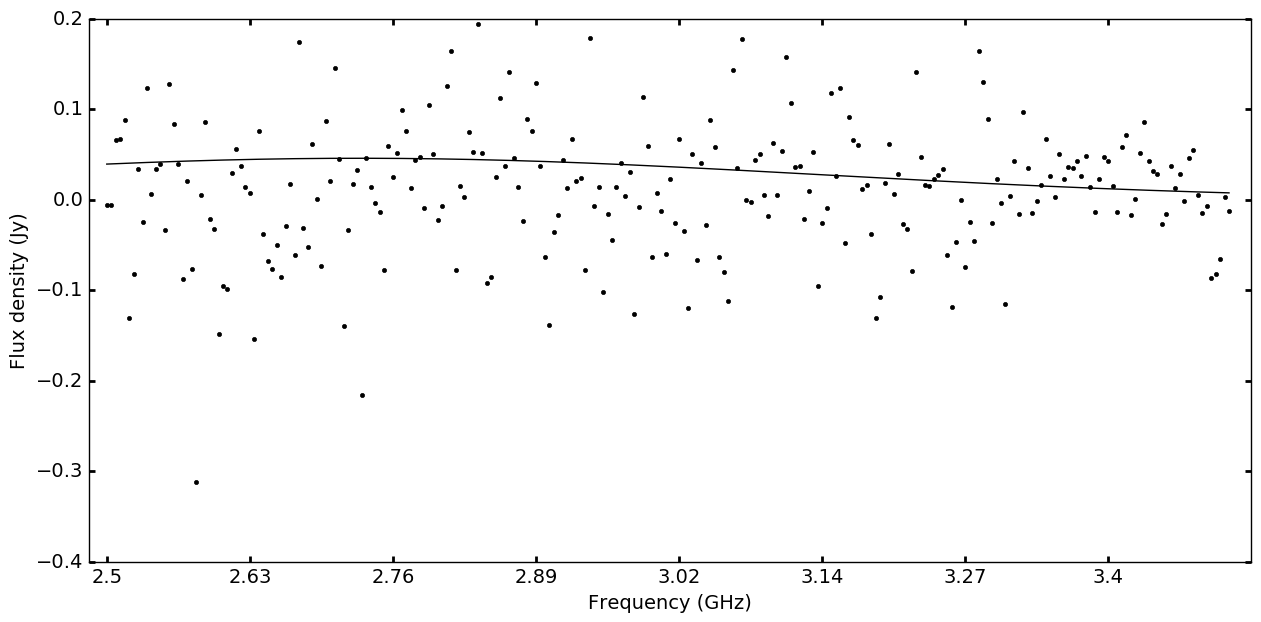
\includegraphics[width=0.3\columnwidth]{spec_57645.png}
 \end{minipage}

 \begin{minipage}{2\columnwidth}
  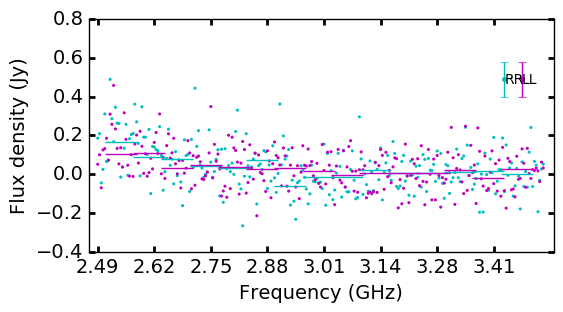
\includegraphics[width=0.3\columnwidth]{spec_57646.png}
  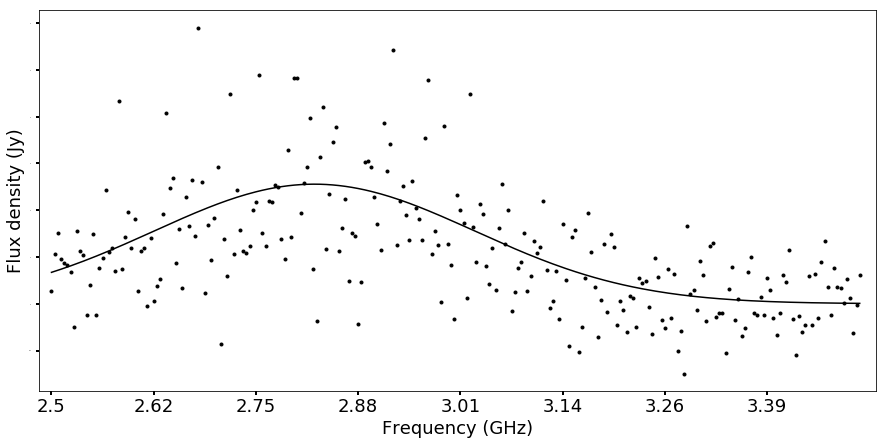
\includegraphics[width=0.3\columnwidth]{spec_57648.png}
  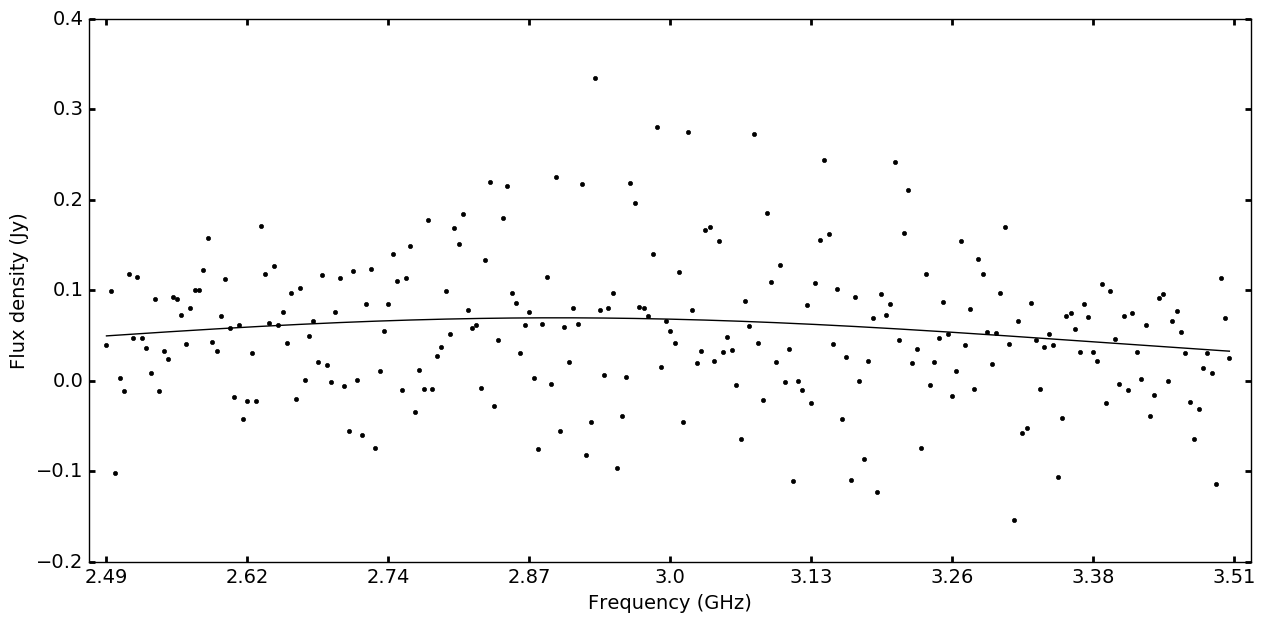
\includegraphics[width=0.3\columnwidth]{spec_57649.png}
 \end{minipage}
\caption{Spectra of nine bursts seen by the VLA from 2.5 to 3.5~GHz.  **LABELS ALL SAME FREQ. SOME SHOULD START HIGHER FOR DROPPED CHANNELS**
%Table?
%57623 (DM$=561$ pc cm$^{-3}$)
%57633, Scan 7 (DM$=554$ pc cm$^{-3}$)
%57633, Scan 13 (DM$=559$ pc cm$^{-3}$)
%57638 (DM$=554$ pc cm$^{-3}$)
%57643 (DM$=559$ pc cm$^{-3}$)
%57645 (DM$=572$ pc cm$^{-3}$)
%57646 (DM$=573$ pc cm$^{-3}$)
%57648 (DM$=559$ pc cm$^{-3}$)
%57649 (DM$=552$ pc cm$^{-3}$).
\label{fig:spec}}
\end{center}
\end{figure*}

We fit a Gaussian model to each burst to estimate their characteristic width and peak flux... As shown in Table \ref{tab:spec}, the typical frequency scale is xx MHz...

\subsubsection{Spectral Autocorrelation}
The spectral autocorrelation is used to infer both intrinsic and scintillation properties \citep{}. Figure \ref{fig:acf} shows the spectral autocorrellation for the MJD 57633, scan 7 burst. Some marginal evidence of spectral correlation on the scale of the channel resolution (4~MHz)?

\begin{figure}[htb]
\begin{center}
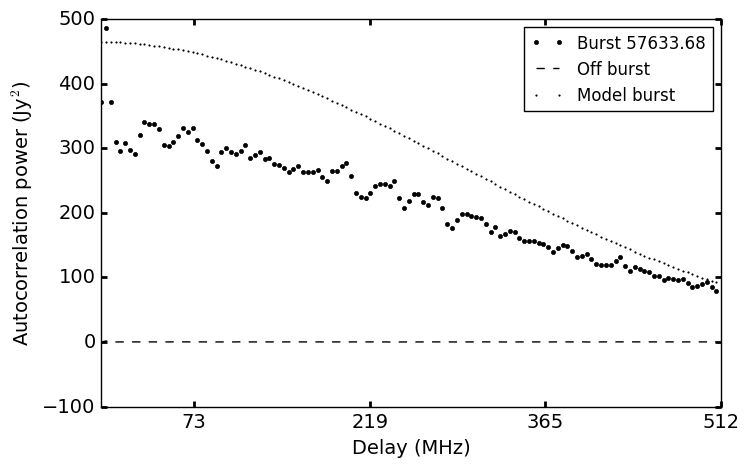
\includegraphics[width=0.9\columnwidth]{acf_57633_scan7}
\caption{
\label{fig:acf}}
\end{center}
\end{figure}

\subsubsection{Circular Polarization}
The VLA S-band recievers natively measure circular polarization, although observations did not include polarization calibration procedures. Crude constraints on circular polarization are possible by comparing the burst intensity in right and left-hand polarized data products. The apparent circular polarization fraction ($(RR-LL)/(RR+LL)$) for the most significant bursts are all less than 3\%. FRB121102 was located 2.3 arcmin away from pointing center, where systematic effects have been measured as large as 3\% (Perley et al 2016, VLA memo). We conclude that the S-band bursts seen by the VLA have a circular polarization of less than 3\%.

\subsection{Multi-Telescope Burst Spectra}
See Figure \ref{fig:multi} for coverage of VLA bursts... Arecibo had coverage for 57648 VLA burst and sees a coincident burst. No other coincident bursts seen. **Make figure of VLA/AO dynamic spectrum on 57648**

%\begin{figure}[htb]
%\begin{center}
%\includegraphics[width=0.9\columnwidth]{}
%\caption{
%\label{fig:}}
%\end{center}
%\end{figure}

Given measured band for VLA/AO detection/limits, plus in-band VLA detections, we can characterize typical burst spectrum as an envelope of width xx MHz. The center frequency can fall at any GHz band.

\subsection{Brightness Distribution}

The bursts seen by the VLA range in significance from 10 to 150$\sigma$. Table \ref{tab:spec} shows the estimated burst luminosity from spectral modeling...

Figure \ref{fig:logns} shows the flux distribution of the nine VLA bursts. Quantify flatness...

\begin{figure}[htb]
\begin{center}
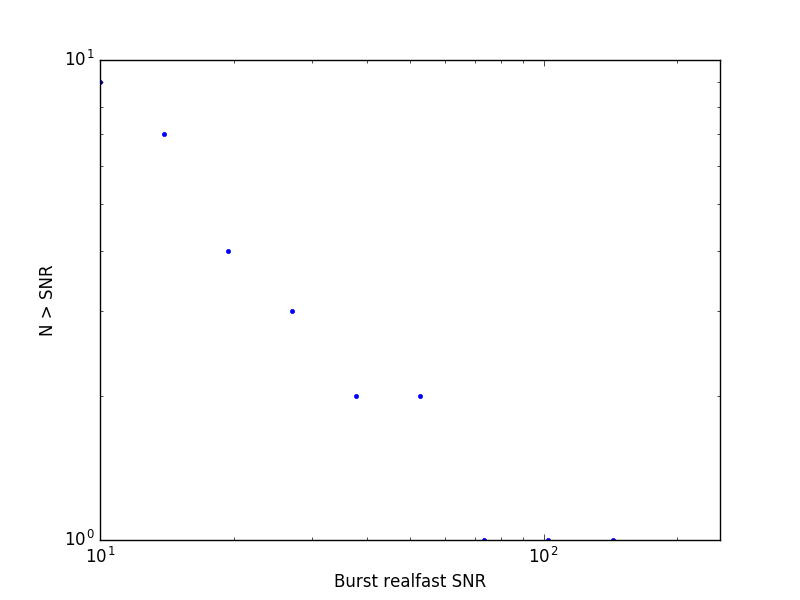
\includegraphics[width=0.9\columnwidth]{logns}
\caption{Log N -- Log SNR distribution of real-time detections of FRB 121102. **Update to luminosity distribution**
\label{fig:logns}}
\end{center}
\end{figure}

Compare luminosity distribution to flux distribution measured by \citep{2016ApJ...830...75V}...

\subsection{Temporal Statistics}
Burst detections were made very inhomogenously though the roughly 63 hours of observing toward FRB 121102. Data quality are relatively high and RFI did not significantly impact sensitivity, so the inhomogeneous burst distribution not an observational artifact.

In the first $\sim25$\ hours observing at S-band no bursts were detected, while nine bursts were detected in the last $\sim30$ hours of S-band observing. Assuming the burst detection probability follows a stationary Poisson distribution, the nondetection in the first half of S-band limits the FRB rate to $\rm{R}<0.12$ hour$^{-1}$. The mean detection rate for the last part of the campaign was $\rm{R}=0.3$ hour$^{-1}$. The inconsistency shows that the detection probability is not stationary.

Moreover, there is weak evidence that the \frb\ burst rate changes during the last part of the campaign. We modeled the event detection probability as a Poisson probability with a rate parameter that scales linearly with time as $R=a + b*(\rm{MJD} - 57623)$. We then calculated the probability of measuring the observed event rate as $\Pi P_i(R)$. Figure \ref{fig:rate} shows the ($a$, $b$) parameter space with contours of 50, 90, and 95\% confidence contours. 

\begin{figure}[htb]
\begin{center}
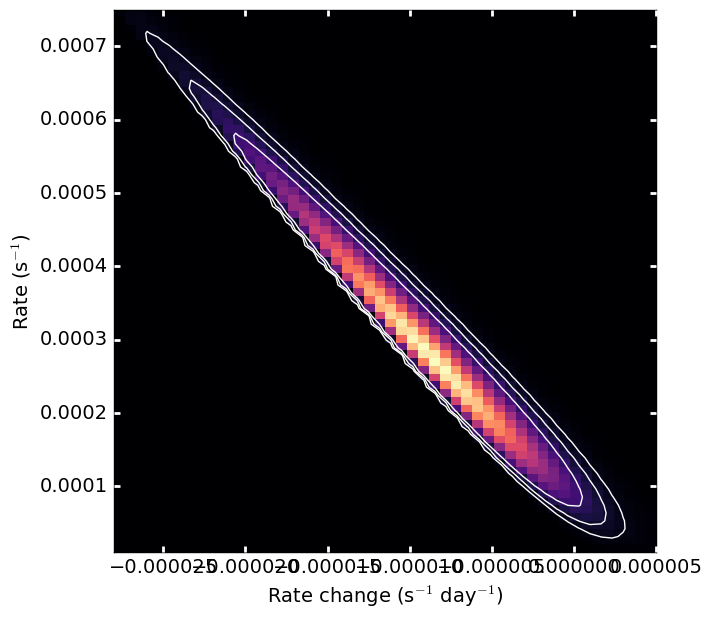
\includegraphics[width=0.9\columnwidth]{event_rate_contours}
\caption{Rate versus rate change during last campaign.
\label{fig:rate}}
\end{center}
\end{figure}

Figure \ref{fig:ls} shows a Lomb-Scargle periodogram...
Lots of excess power corresponding to periods shorter than 1 hour.

\begin{figure}[htb]
\begin{center}
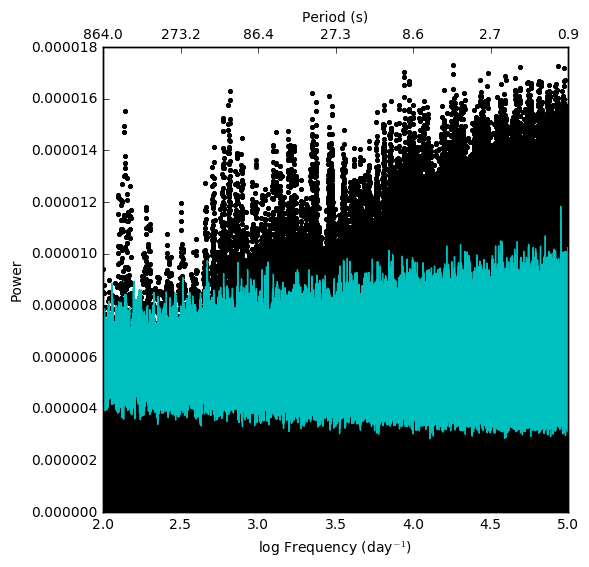
\includegraphics[width=0.9\columnwidth]{lombscargle}
\caption{Lomb-Scargle periodogram with 95\% limit on power from last observing campaign
\label{fig:ls}}
\end{center}
\end{figure}


\section{discussion}

\subsection{Luminosity Distribution}
Doubts were cast on the first FRB detection (``Lorimer burst'') due to its unusually high brightness. The lack of lower-significance detections suggested that this burst was unlikely to be part of any astrophysical population. With more detections, it has become clear that the FRB population has a relatively flat flux distribution \citep{2016ApJ...830...75V, 2016arXiv161100458L}. This fact was demonstrated with yet another detection of an extremely bright FRB \citep{2016arXiv161105758R}.

Discuss comparison FRB 121102 luminosity distribution to that of FRB population...
Imagine physical log N/log S with cut-offs and scattering can bias the intrinsic into the observed distribution (Macquart and Johnston)...


\subsection{Repetition}
Discussion of ``red spectrum'' and \citet{2016MNRAS.458L..89C}. Bursts predict bursts therefore repetition constraints of other FRBs are likely weaker than claimed...

Constraints on repetition assuming "red spectrum" for whole population. Simulation using observed burst temporal statistics...

Intrinsic versus refractive scintillation...

Fewer FRBs out there...

\subsection{Emission Physics and Burst Energetics}

% from first paper
For a nominal Gpc distance $D$ corresponding to redshifts $z\lesssim 0.3$, the received fluence $A_{\nu}$ from each burst implies  a burst energy
$$E_{\rm burst} = 4\pi D^2 (\delta\Omega/4\pi) A_{\nu} \Delta\nu
\approx 10^{38}\, {\rm erg}\,(\delta\Omega/4\pi) D_{\rm Gpc}^2  (A_{\nu} / 0.1\ {\rm Jy\ ms}) \Delta\nu_{\rm GHz}.$$
The unknown  emission solid angle $\delta\Omega$
could be very small due to relativistic beaming, and together with a distance possibly much smaller than 1~Gpc, could reduce the energy requirement significantly.  However, the {\it total} energy emitted could be larger depending on the duration of the emission in the source frame and other model-dependent details.
Either way, the burst energies from \frb\ are not inconsistent with those that might be expected from the magnetosphere of a compact object\cite{cw16}.



\subsection{Observing Strategies}

Repetition implies that targeting known FRBs is optimal.

Repetition and shallow luminosity distribution show that shallow and wide is the best way to blindly find FRBs.

Given that bursts have $<1$~GHz-scale spectra, wide bandwidths improve odds of detection.

\section{Conclusions}



\bibliographystyle{apj}

\section*{Acknowledgements}
We thank ...
This project was supported by the University of California Office of the President under Lab Fees Research Program Award 237863. The National Radio Astronomy Observatory is a facility of the National Science Foundation operated under cooperative agreement by Associated Universities, Inc.. This research made use of Astropy, a community-developed core Python package for Astronomy (Astropy Collaboration, 2013).

\bibliography{fasttrants.bib}

%\begin{figure}[htb]
%\begin{center}
%\includegraphics[width=0.9\columnwidth]{}
%\caption{
%\label{fig:name}}
%\end{center}
%\end{figure}

%\begin{table}
%\caption{Caption}
%\footnotesize
%\centering
%\begin{tabular}{l|cc|cc|c}
%\hline
%Field       & RA          & Dec   & Lon. & Lat.     & Time \\
%            & \multicolumn{2}{|c|}{(J2000)}  & \multicolumn{2}{|c|}{(Galactic; deg)} & (hrs) \\ \hline
%RA02        & 2:27:53  &  +9:13:24 & 159.0 & --46.8    & 26.25 \\
%PSR J2248-0101 & 22:48:27 & --1:1:48 & 69.3 & --50.6 & 6.5 \\ \hline
%\end{tabular}
%\label{fields}
%\end{table} 

\end{document}

